\newpage
% TODO: ТУТ ВСЕ НАДО ПОМЕНЯТЬ НА СВОЕ!!!
\section{Обработка результатов измерений}
\subsection{Влияние разрешения на вид спектра}
Для начала изобразим вид опорного спектра (без колбы) при разном разрешении (рис. \ref{resolution}).
%\begin{figure}[h!]
%	\centering
%	\includegraphics[angle = 90, height=0.84\textheight]{resolution}
%	\caption{Опорный спектр при различном разрешении}
%	\label{resolution}
%\end{figure}



\begin{figure}[h]
	\begin{minipage}[h]{0.5\linewidth}
		\centering
		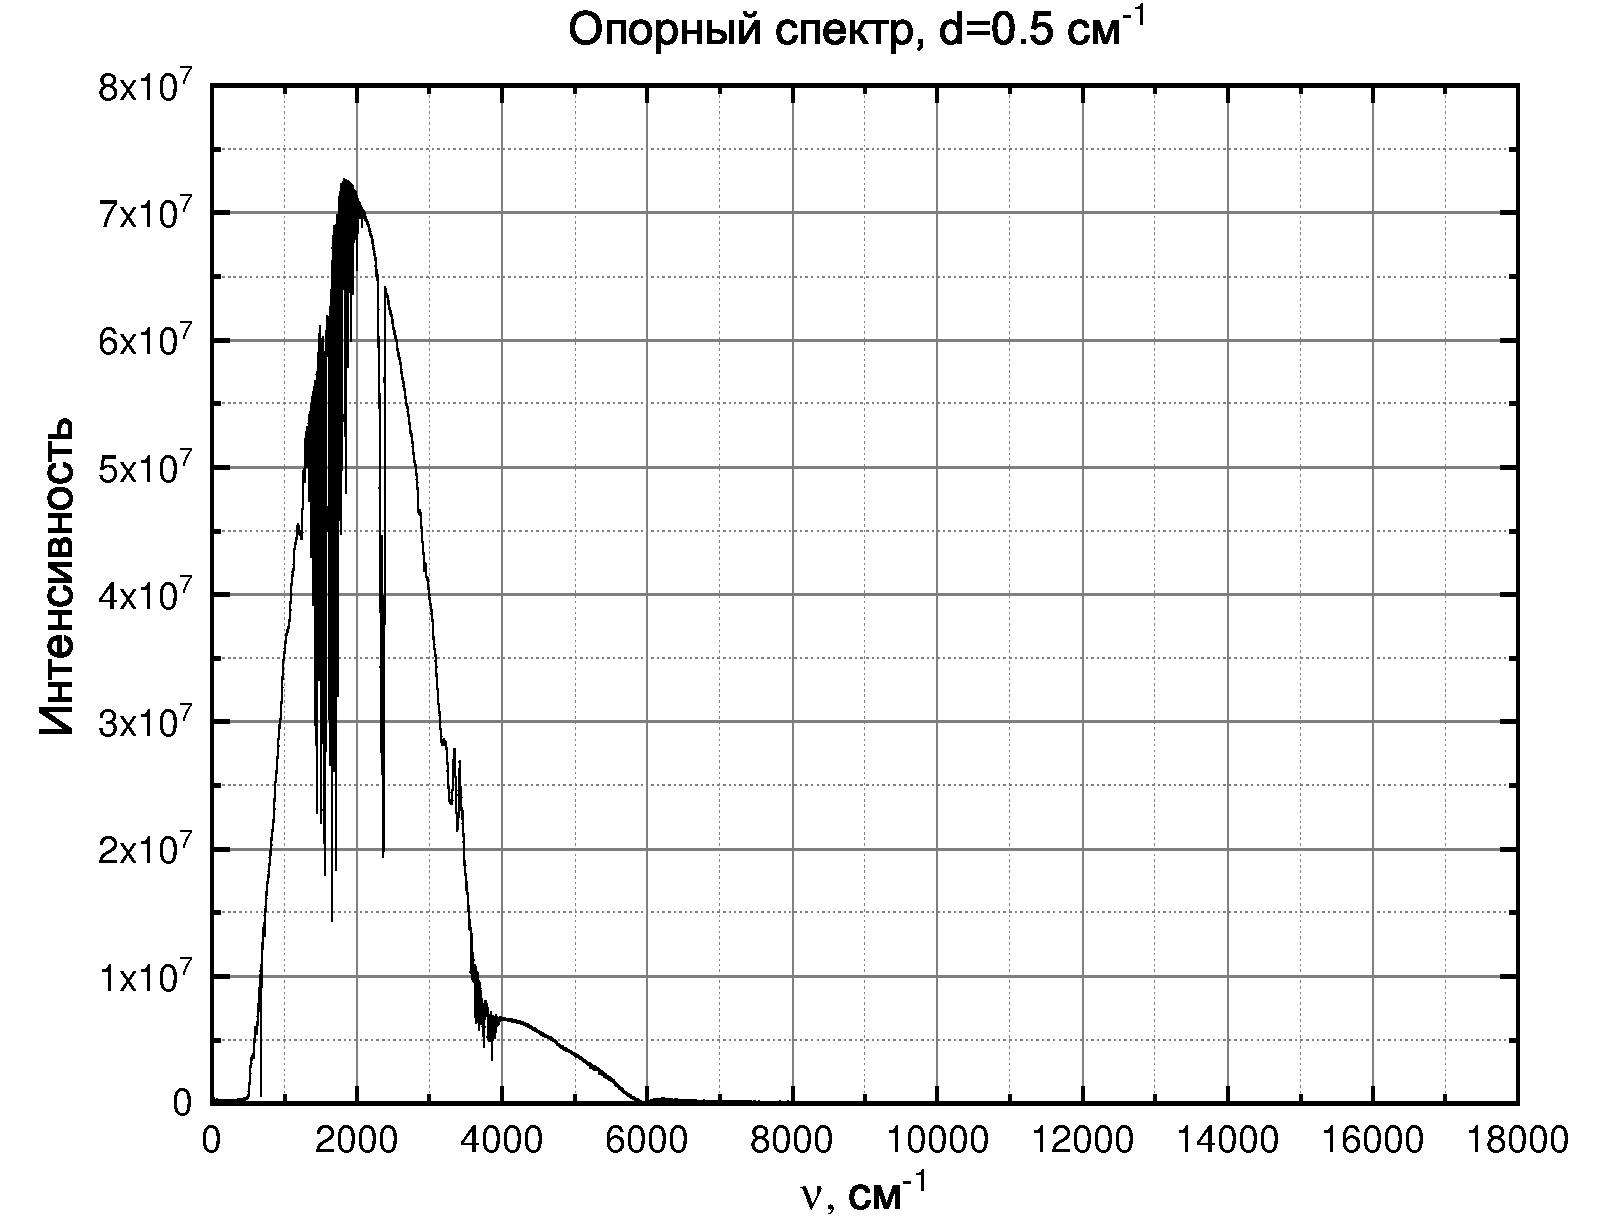
\includegraphics[width=1\linewidth]{data/opor_0_5}
	\end{minipage}
	\begin{minipage}[h!]{0.5\linewidth}
		\centering
		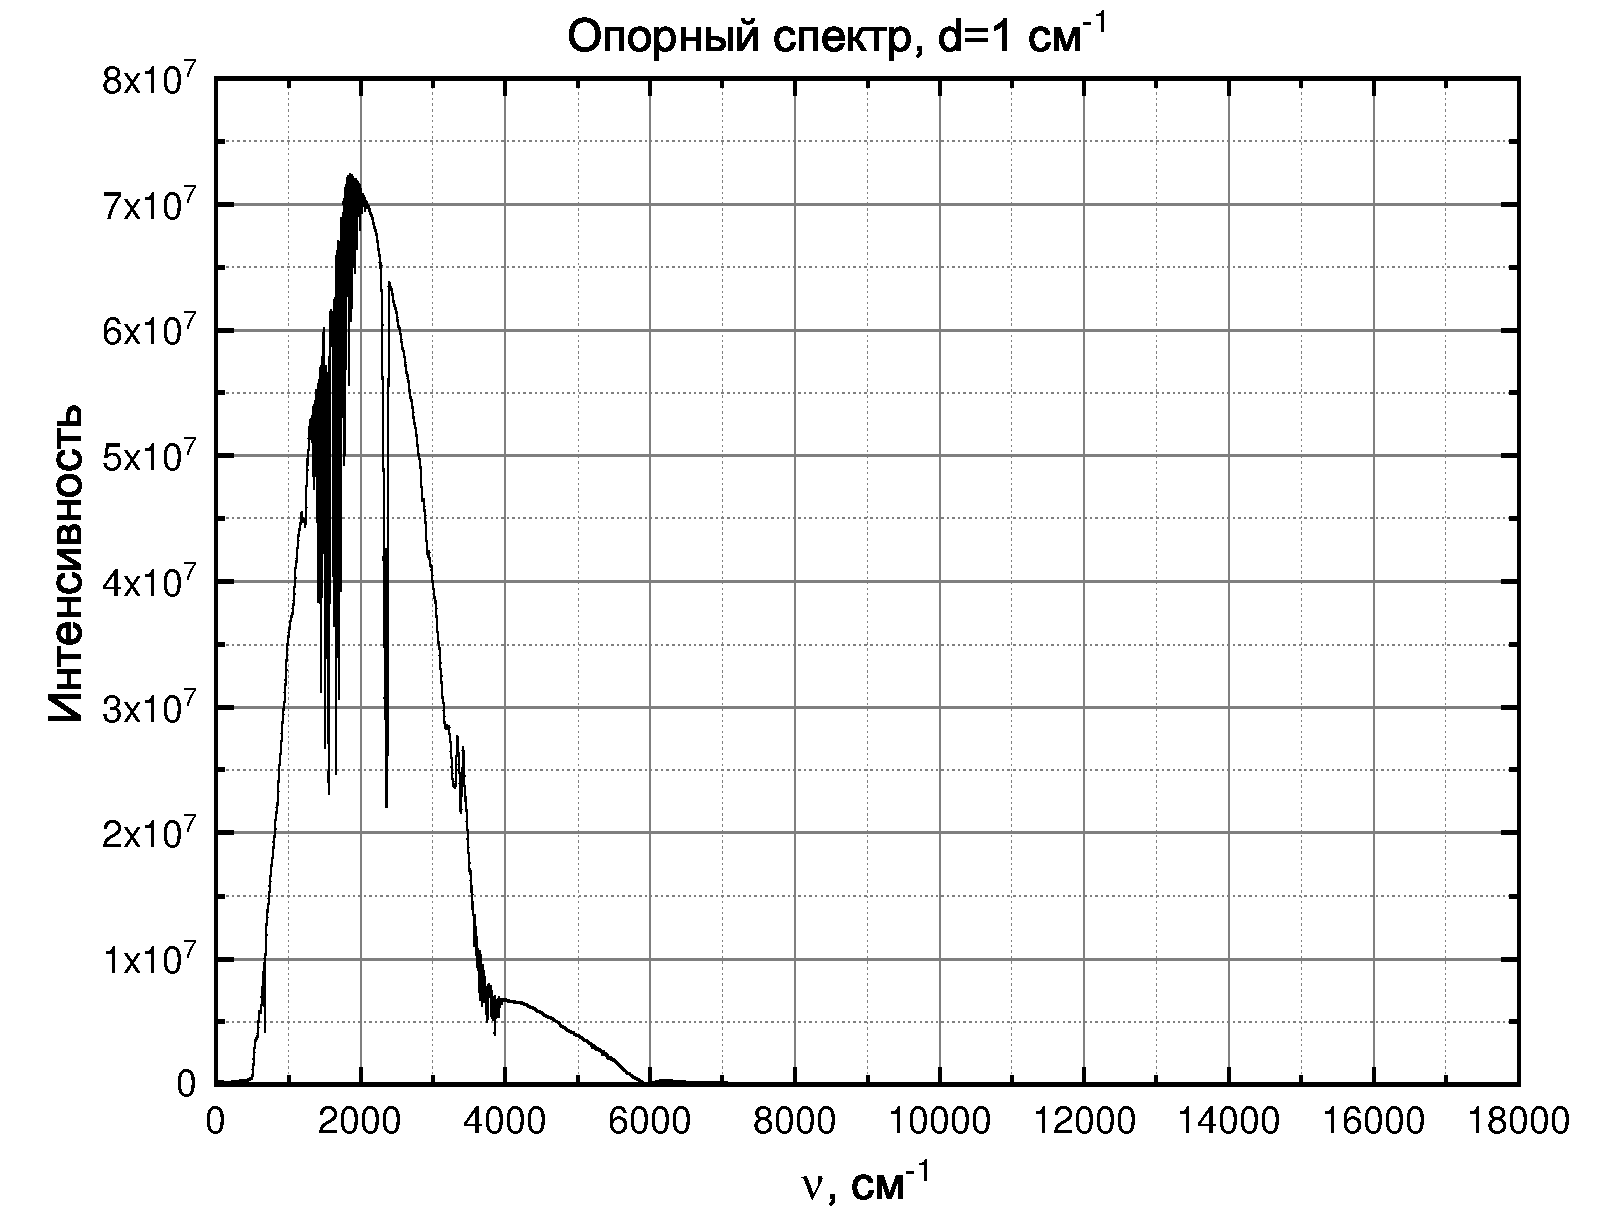
\includegraphics[width=1\linewidth]{data/opor_1}
	\end{minipage}
	\begin{minipage}[h!]{0.5\linewidth}
		\centering
		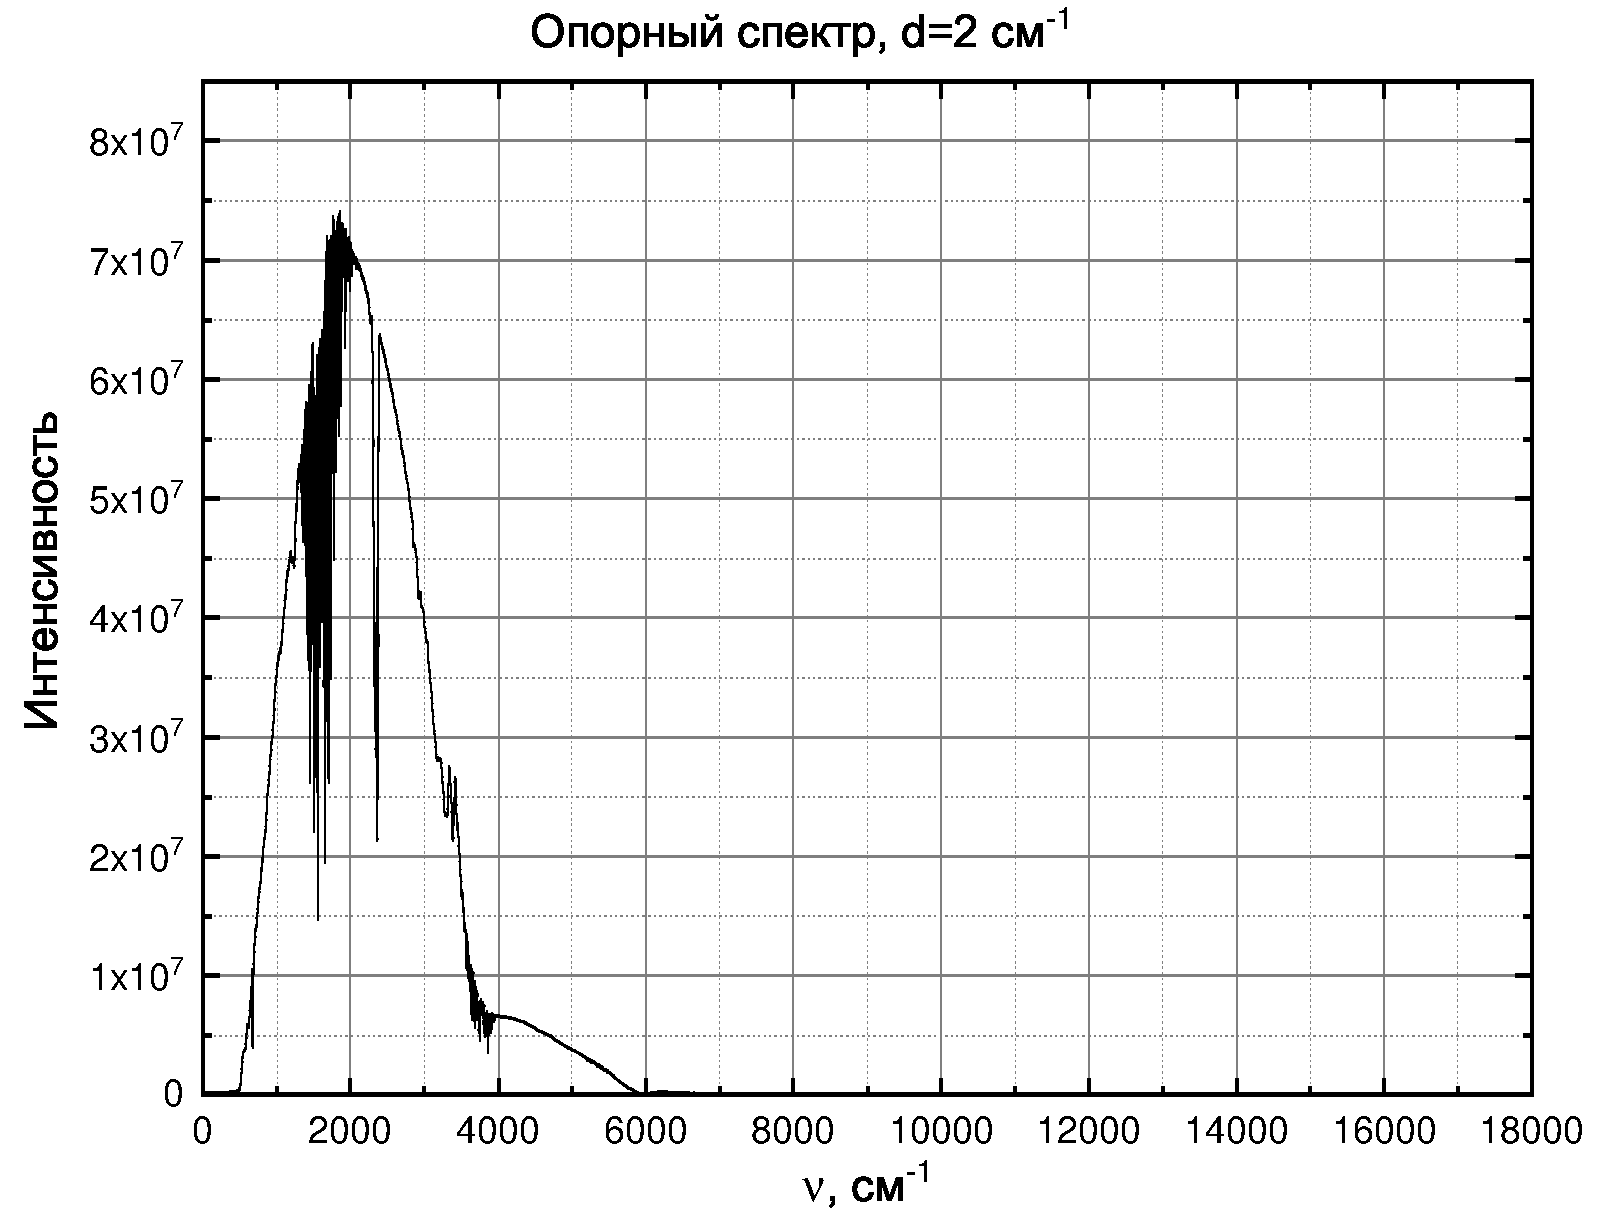
\includegraphics[width=1\linewidth]{data/opor_2}
	\end{minipage}
	\begin{minipage}[h!]{0.5\linewidth}
		\centering
		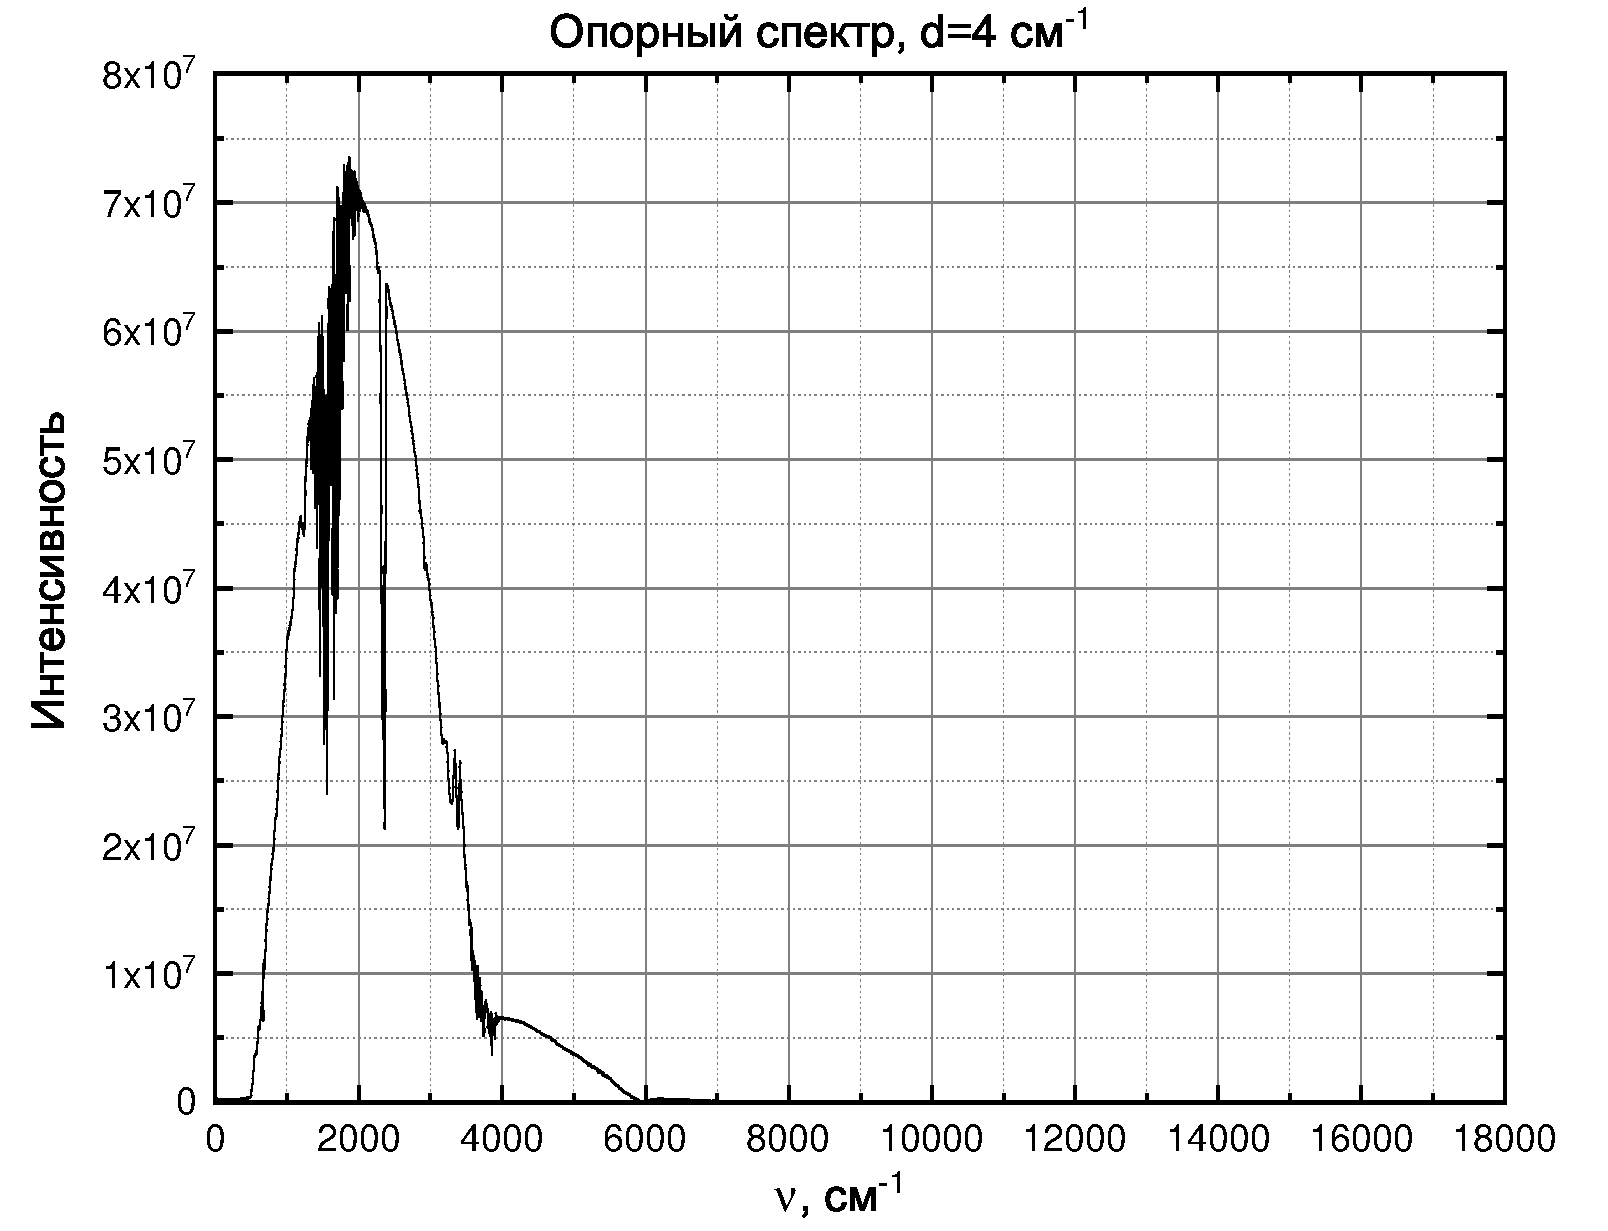
\includegraphics[width=1\linewidth]{data/opor_4}
	\end{minipage}
	\caption{Опорный спектр при различном разрешении}
	\label{resolution}
\end{figure}





Как видно на примере $\nu \approx 1300 \text{ см}^{-1}$, при увеличении разрешения мы хуже разрешаем спектральную картину.
\subsection{Влияние аподизации на вид спектра}
Изобразим на примере двух пиков из опорного спектра, взятых при разном разрешении прибора, как влияет на спектр вид аподизации (рис. \ref{apotis}).

Как видно, треугольная аподизация уширяют пик (падает разрешающая способность), однако остаточные колебания уменьшаются. Более того, при разрешении $4 \text{ см}^{-1}$ остаточные пики и вовсе пропадают.

\begin{figure}[H]
	\centering
	\begin{minipage}[h!]{0.9\linewidth}
		\centering
		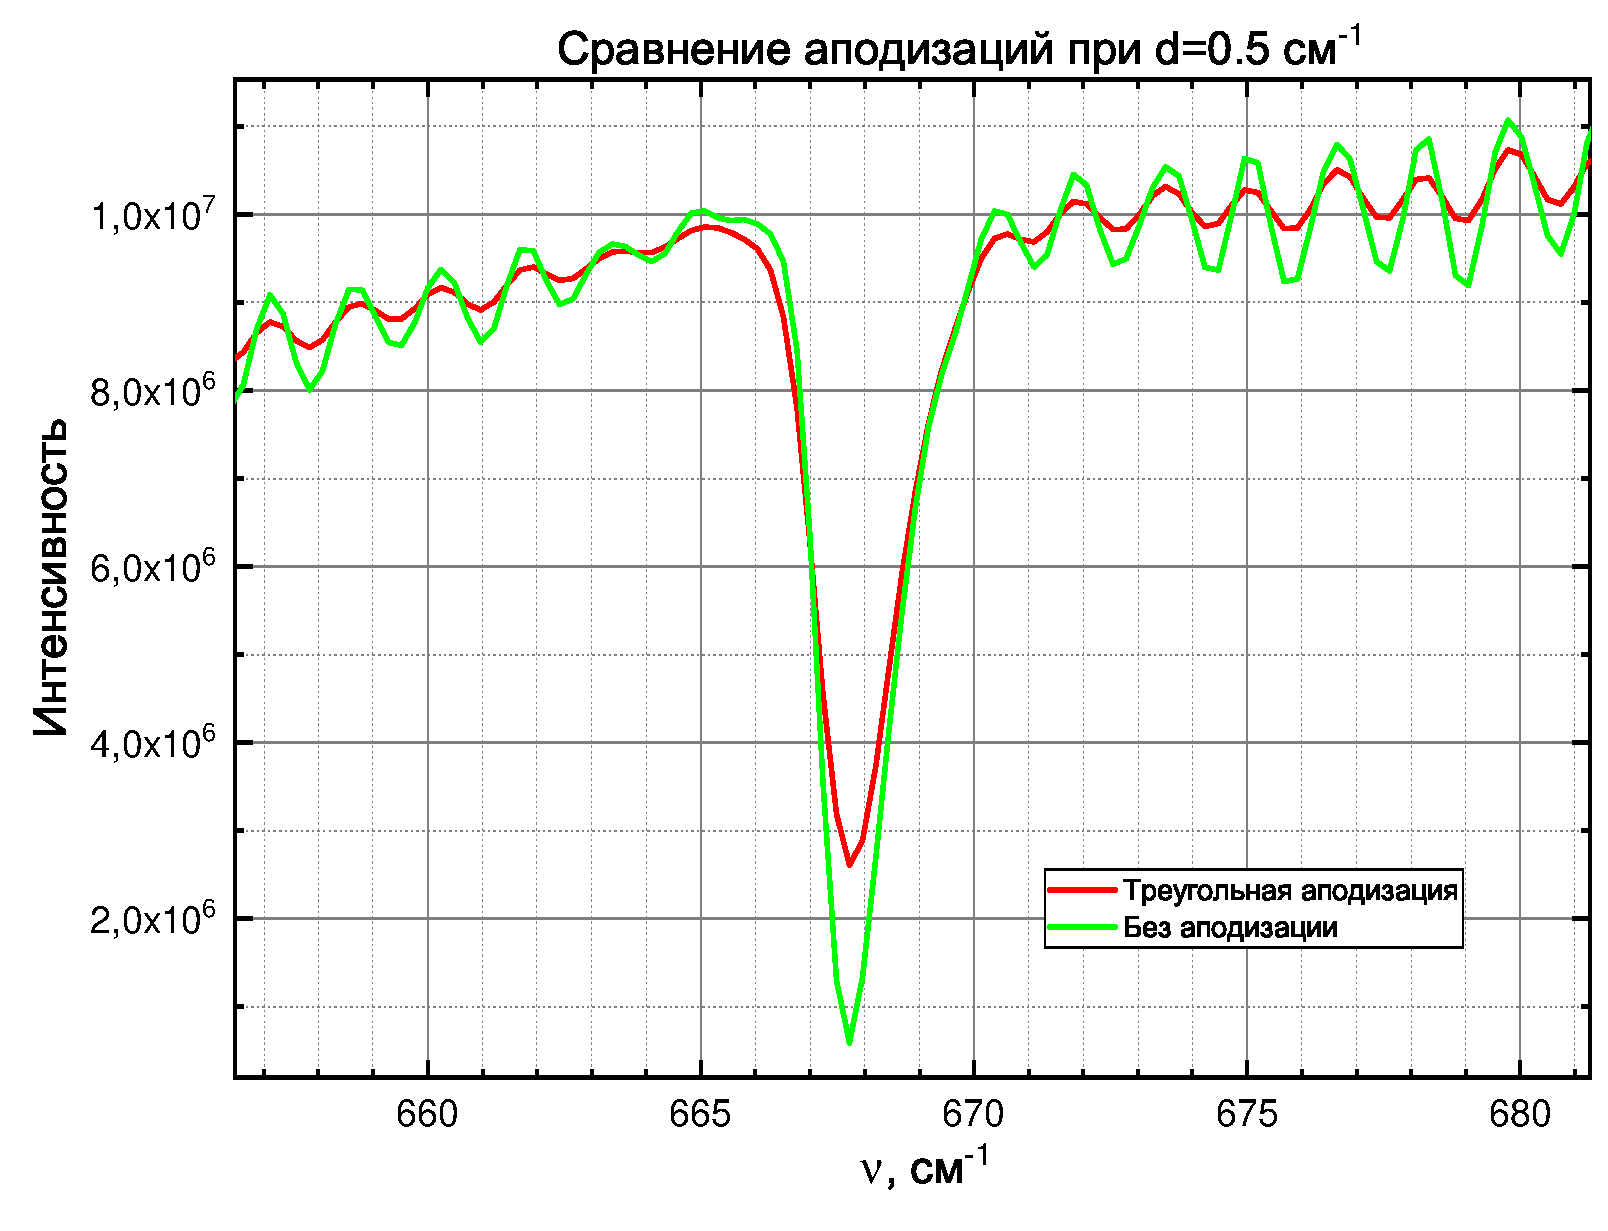
\includegraphics[width=1\linewidth]{data/apodiz_comparation_0_5}
	\end{minipage}\\
	\begin{minipage}[h!]{0.9\linewidth}
		\centering
		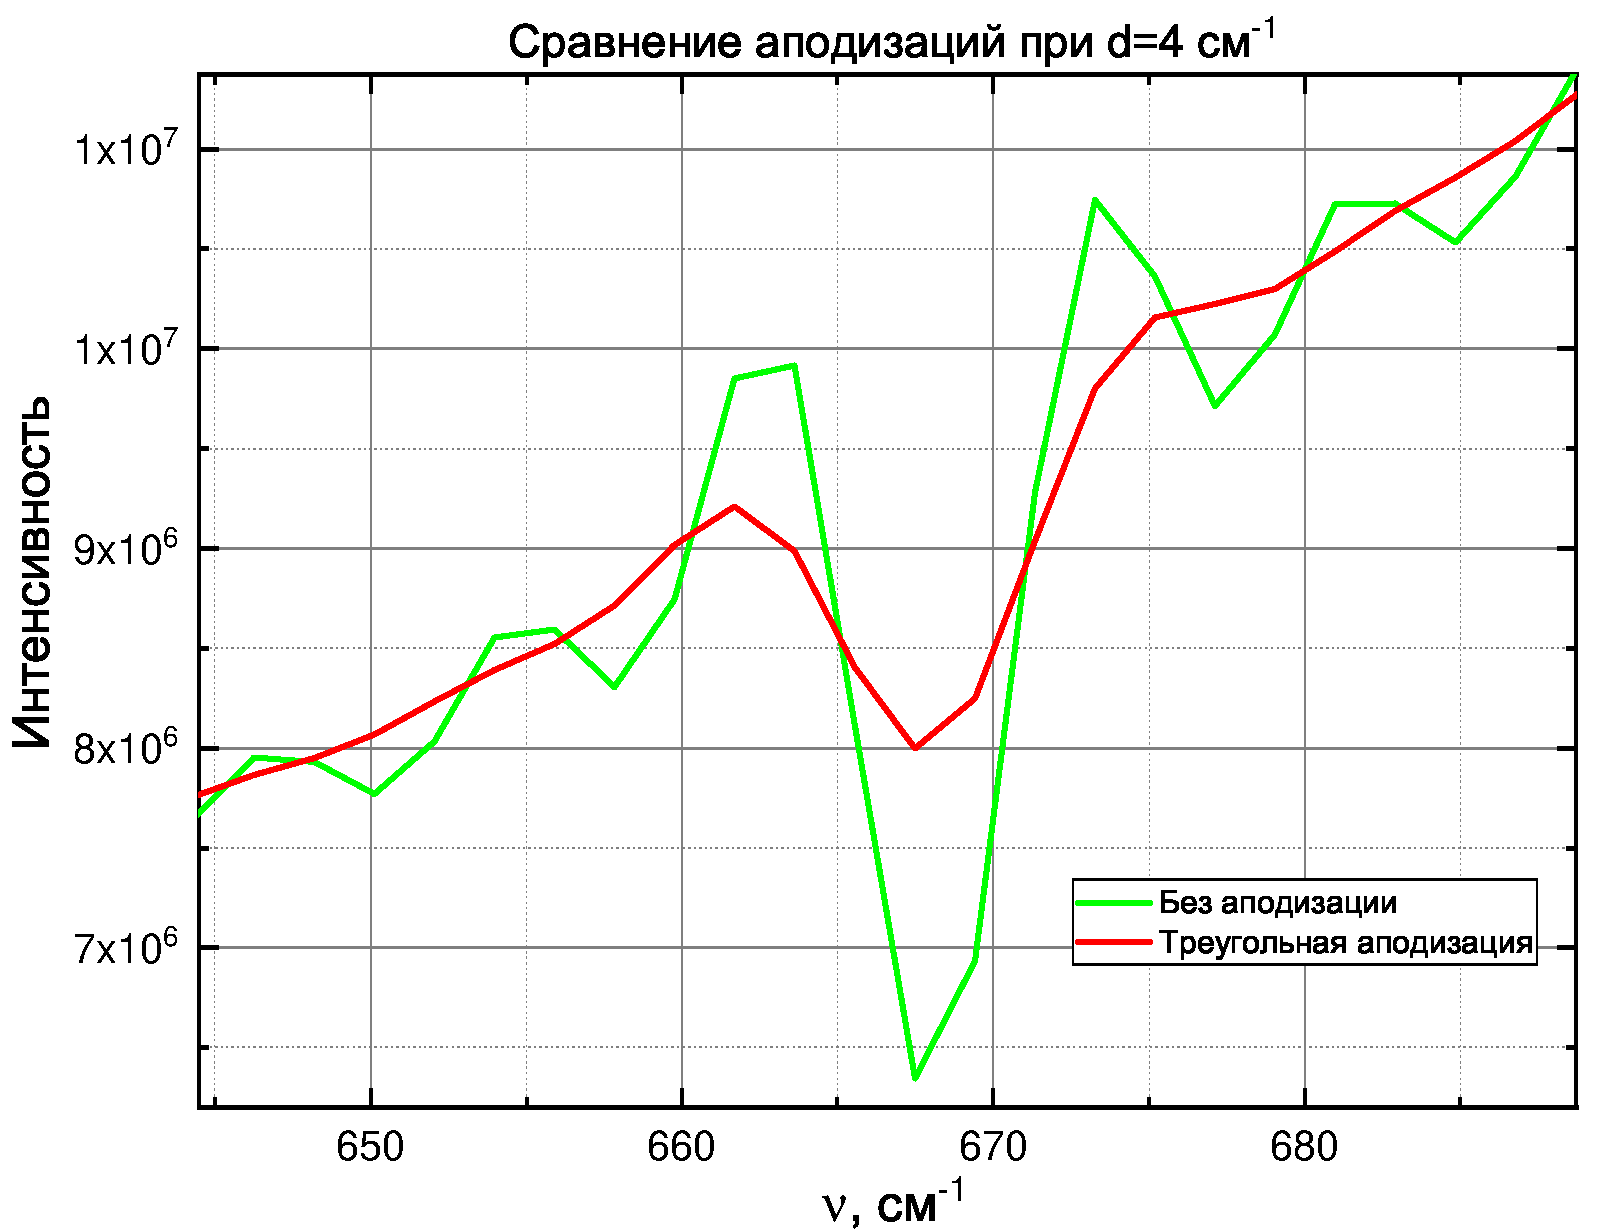
\includegraphics[width=1\linewidth]{data/apodiz_comparation_4}
	\end{minipage}
	\caption{Опорный спектр при различном разрешении}
	\label{apotis}
\end{figure}

\subsection{Спектр пустой кюветы}
Зарегистрируем спектр пустой кюветы (рис. \ref{fig:empty_kvartz}).

\begin{figure}[H]
	\centering
	\vspace{-1.5cm}
	%	\hspace{-1.2cm}
	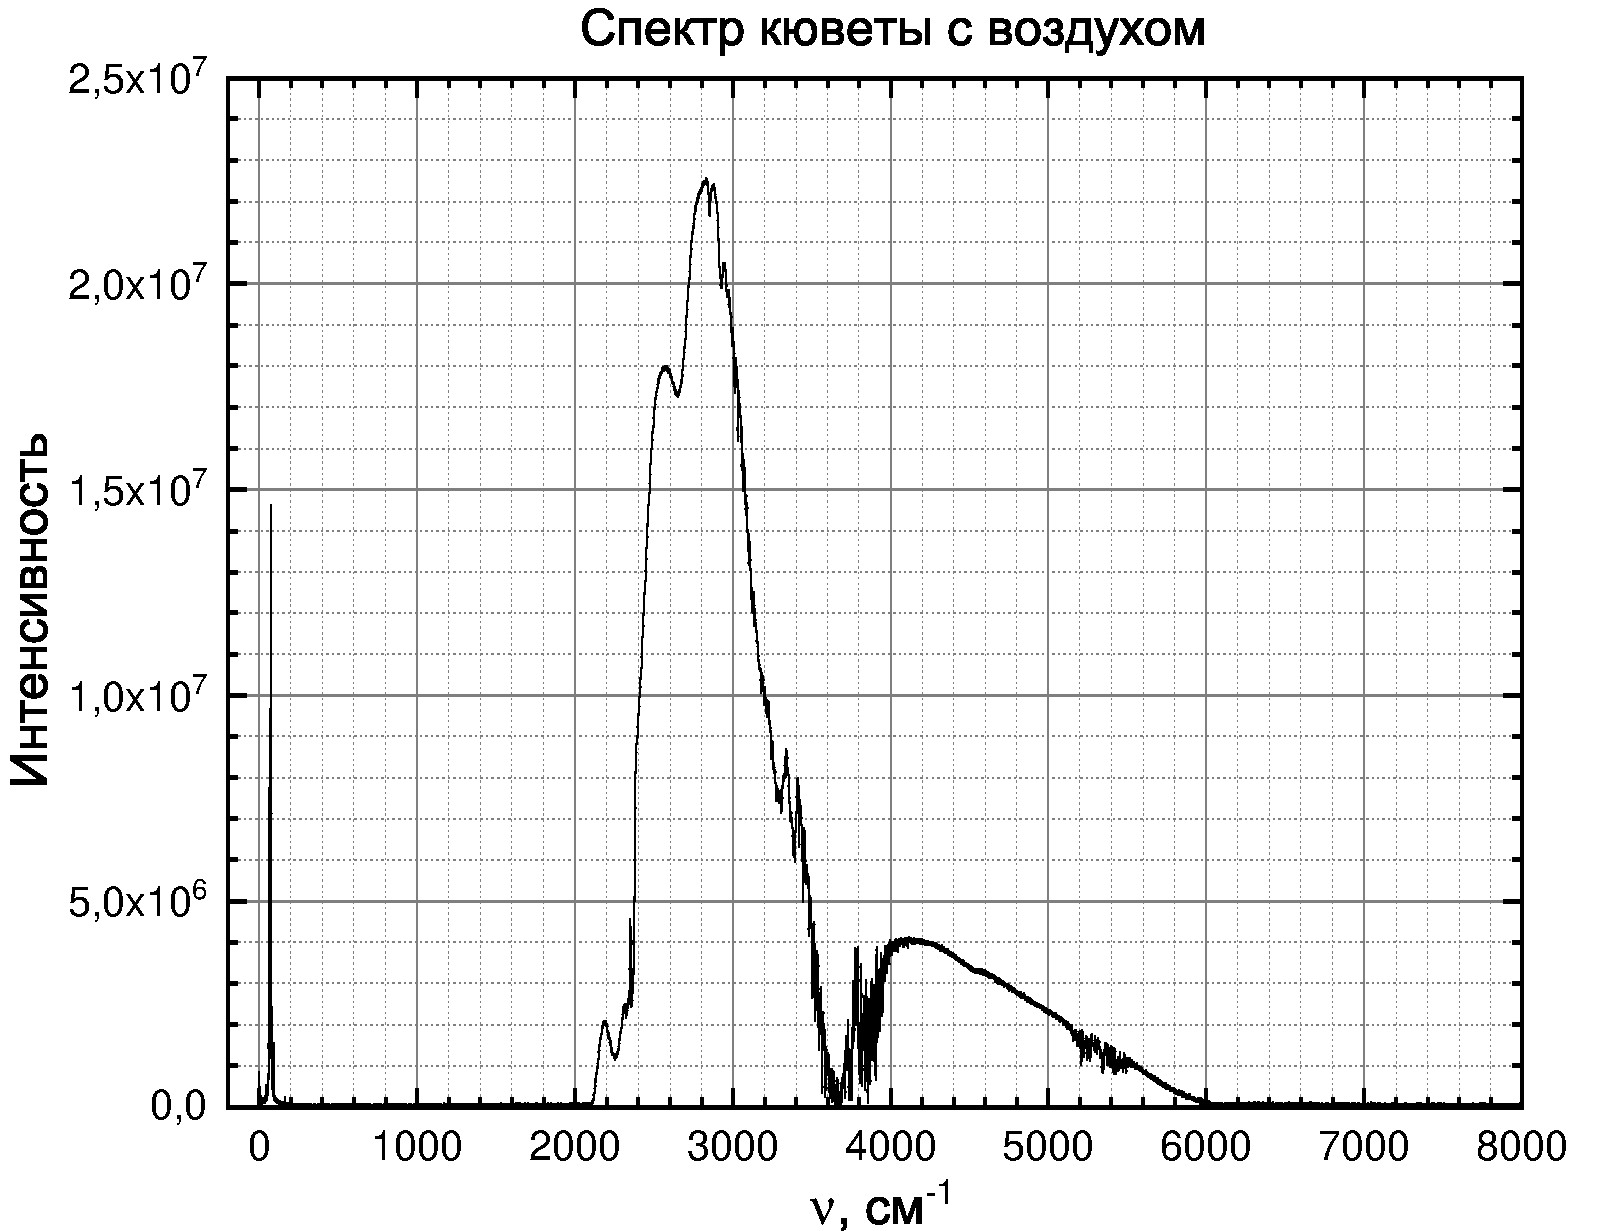
\includegraphics[angle = 90, height=0.85\textheight]{data/vozdyh_kvartz}
	\caption{Спектр пустой кюветы с воздухом}
	\label{fig:empty_kvartz}
\end{figure}

В ходе эксперимента не удалось полностью избавиться от воды в кювете, поскольку предыдущие экспериментаторы не почистили ее за собой (\textit{мудаки, короче}) и нам пришлось ее промывать непосредственно перед экспериментом. Из-за этих непредвиденных обстоятельств колба не успела до конца просохнуть, что и отразилось на структуре спектра.

\subsection{Молекула HCl}
Изобразим колебательно-вращательный спектр молекулы HCl (рис. \ref{HCL_spec}). Для вычитания базовой линии, нахождения и фитирования пиков был использован пакет Origin.

\begin{figure}[H]
	\centering
%	\hspace{-1.2cm}
	\includegraphics[angle = 90, height=0.88\textheight]{data/HCL_peaks}
	\caption{Колебательно-вращательный спектр молекулы HCl}
	\label{HCL_spec}
\end{figure}

% TODO: подсчитать СВОИ константы

Для определения вращательных постоянных $B_0$ и $B_1$ из
колебательно-вращательных спектров используются так называемые
комбинационные разности $\Delta_2F(j)$, которые представляют собой разность энергий двух вращательных состояний, расположенных через
один вращательный уровень. Можно показать, что разности
\begin{equation}
\label{eq:deltaF'}
\Delta_2F'(j)=F'(j+1)-F'(j-1)=\nu_R(j)-\nu_P(j)
\end{equation}
\begin{equation}
\label{eq:deltaF''}
\Delta_2F''(j)=F''(j+1)-F''(j-1)=\nu_R(j-1)-\nu_P(j+1)
\end{equation}
связаны с вращательными постоянными $B_0$ и $B_1$ следующим образом (не учитываем центробежный член)
\begin{equation}
\label{eq:deltaF'B}
\Delta_2F'(j)=4B_1(j+\frac{1}{2})
\end{equation}
\begin{equation}
\label{eq:deltaF''B}
\Delta_2F''(j)=4B_0(j+\frac{1}{2}),
\end{equation}
где $j$ --- нижний вращательный уровень.

Определим графически постоянные $B_0$ и $B_1$. Этого построим следующие зависимости (рис. \ref{deltaF'} и \ref{deltaF''}).

\begin{figure}[h!]
	\centering
%	\includegraphics[height=0.5\textheight]{deltaF'}
	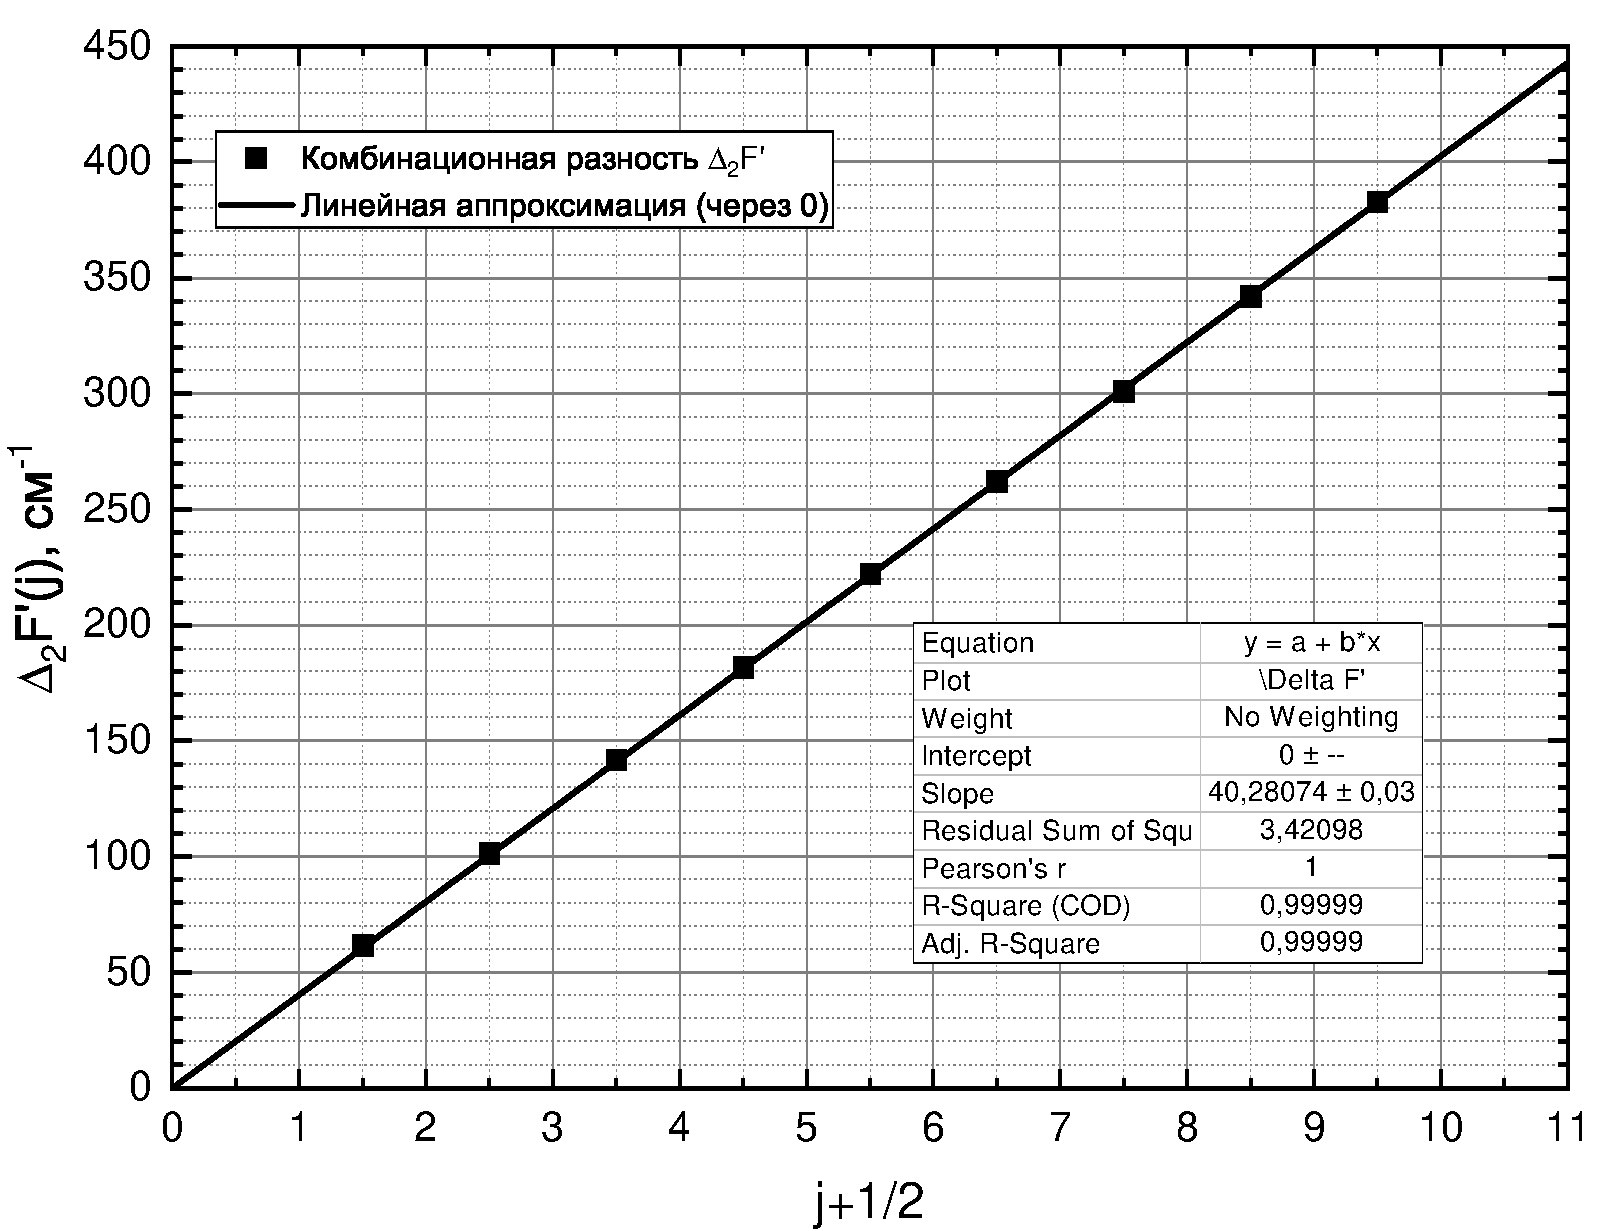
\includegraphics[height=0.5\textheight]{data/delta_F'}
	\caption{Комбинационная разность $\Delta_2F'(j)$}
	\label{deltaF'}
\end{figure}
\begin{figure}[h!]
	\centering
%	\includegraphics[height=0.4\textheight]{deltaF''}
	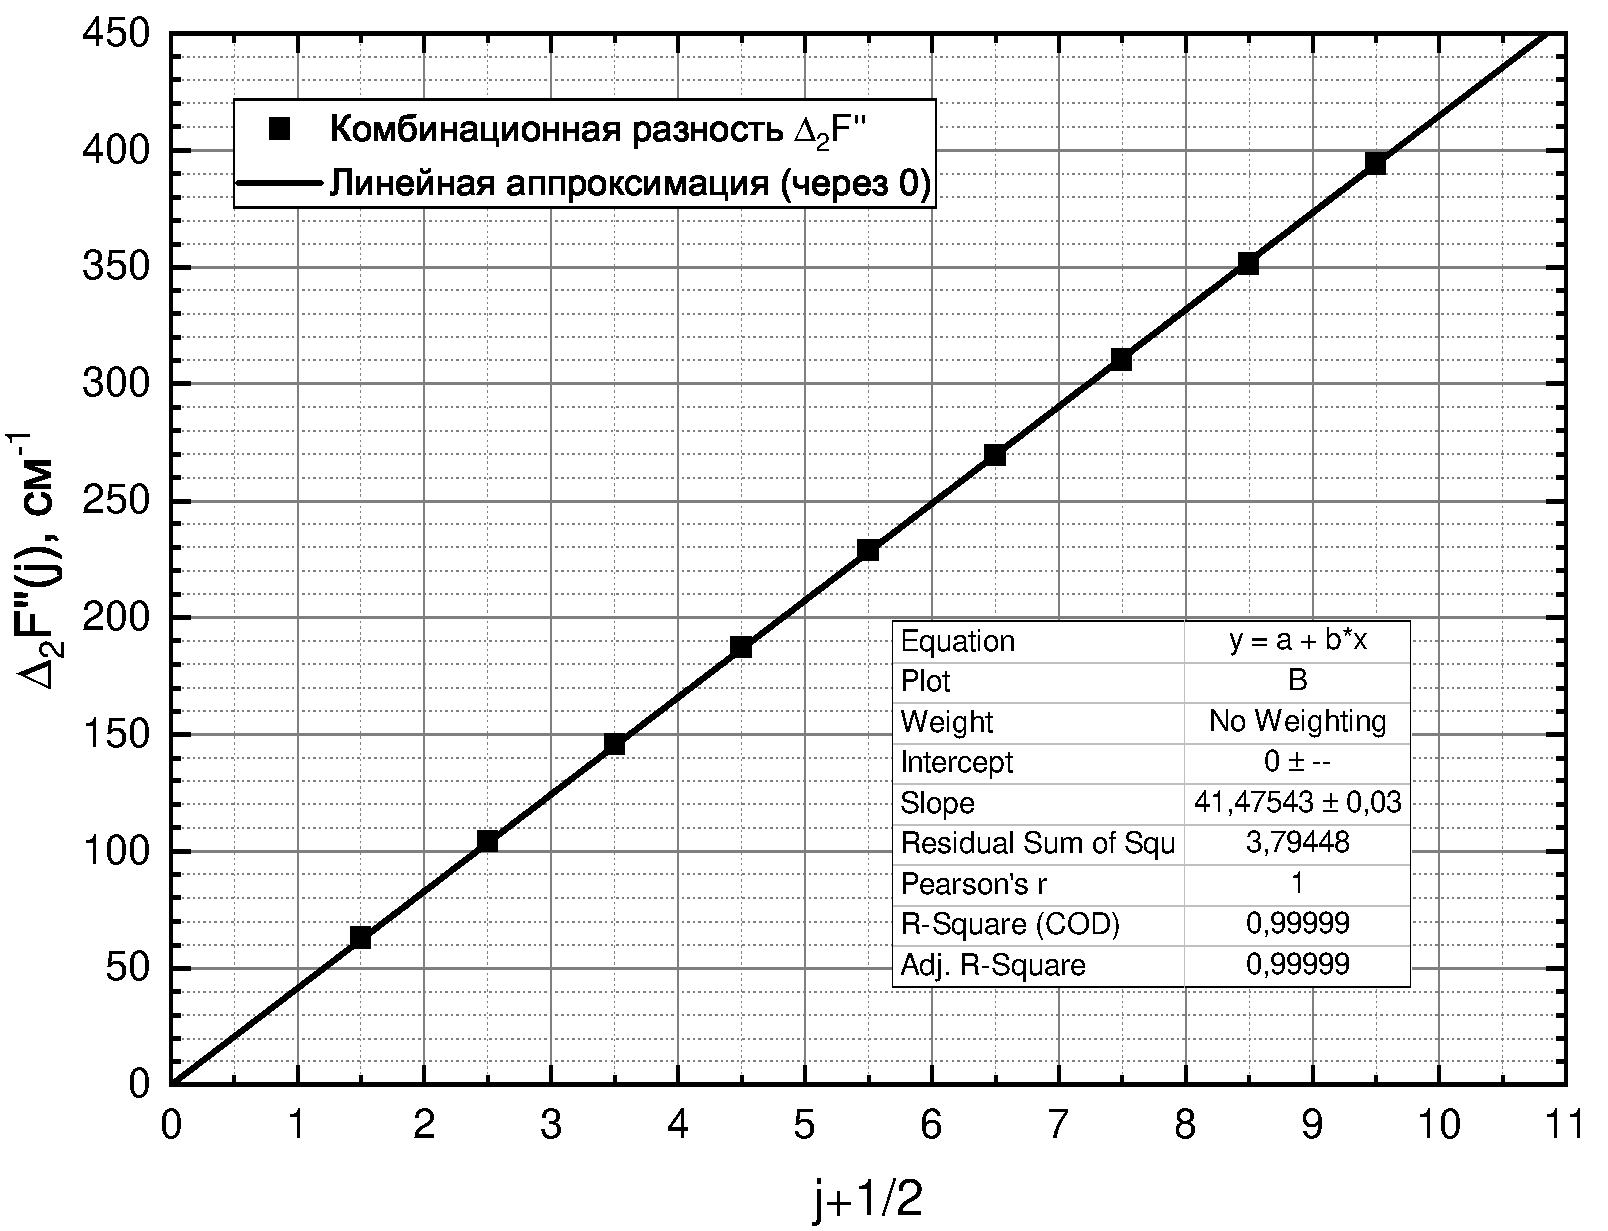
\includegraphics[height=0.5\textheight]{data/delta_F''}
	\caption{Комбинационная разность $\Delta_2F''(j)$}
	\label{deltaF''}
\end{figure}

Откуда получаем
\begin{equation}
B_0 = \dfrac{40.28 \pm 0.03}{4} \text{ см}^{-1} = 10.070 \pm 0.008 \text{ см$^{-1}$}
\end{equation}
\begin{equation}
B_1 = \dfrac{41.48 \pm 0.03}{4} \text{ см}^{-1} = 10.369 \pm 0.008 \text{ см$^{-1}$}
\end{equation}
Отсюда можно найти среднее значение $\omega_e(1-2\chi_e)$
\begin{equation}
\omega_e(1-2\chi_e) = 
2858.56
\text{ см$^{-1}$}
\end{equation}
Воспользуемся табличными данными для волнового числа первого обертона $$2\omega_e(1-3\chi_e) = 5667.98 \text{ см$^{-1}$},$$ откуда
\begin{equation}
\omega_e = 
2907.7
 \text{ см$^{-1}$}
\end{equation}
\begin{equation}
\chi = 
0.008
\end{equation}

Для легких молекул, а также для больших значений $j$ необходимо учитывать постоянную центробежного растяжения $D$ и тогда
\begin{equation}
\Delta_2F(j)=(4B-6D)\left(j+\frac{1}{2}\right)-8D\left(j+\frac{1}{2}\right)^3\approx4B\left(j+\frac{1}{2}\right)-8D\left(j+\frac{1}{2}\right)^3.
\end{equation}
Для практических вычислений удобно воспользоваться преобразованным выражением 
\begin{equation}
\cfrac{\Delta_2F(j)}{\left(j+\frac{1}{2}\right)}=4B-8D\left(j+\frac{1}{2}\right)^2.
\end{equation}
Итак, построим нужные зависимости (рис. \ref{deltaF'_j}, \ref{deltaF''_j}).
%\vspace{5cm}
\begin{figure}[H]
	\vspace{-0.8cm}
	\centering
%	\includegraphics[height=0.49\textheight]{deltaF'_j_05}
	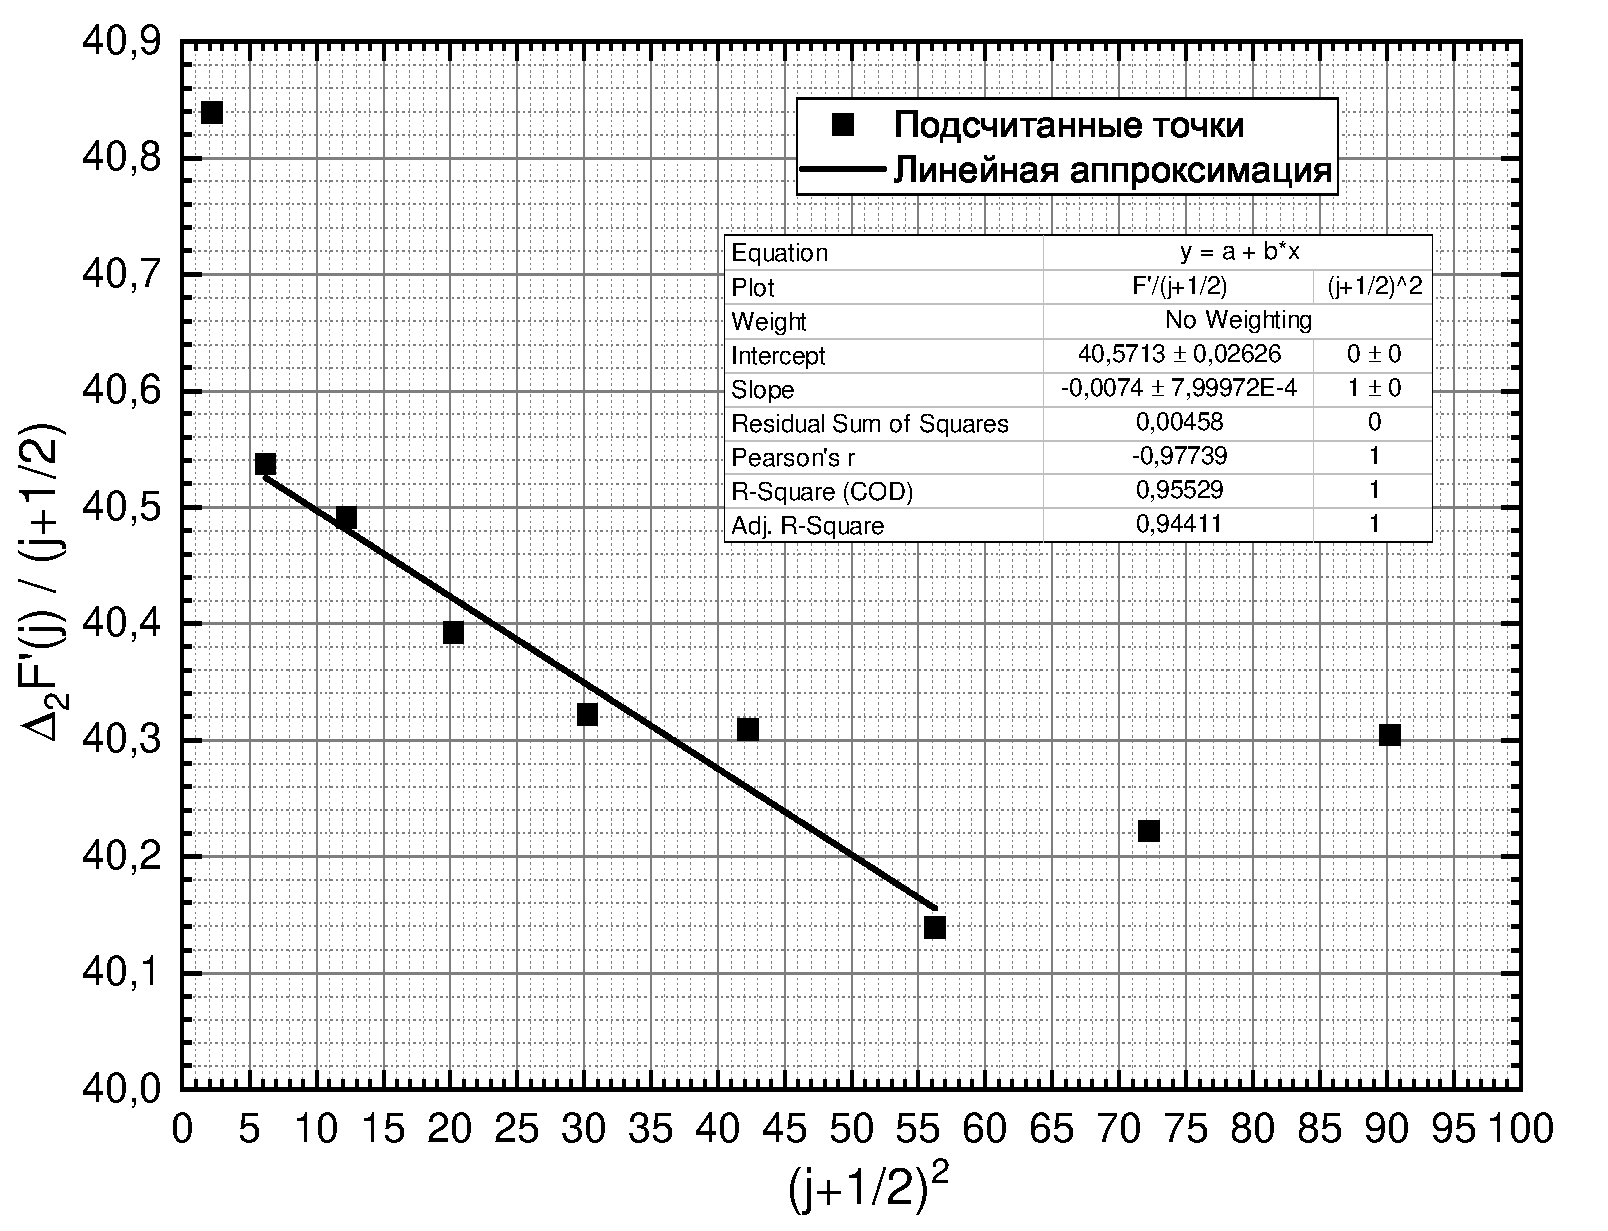
\includegraphics[height=0.49\textheight]{data/delta_F'_j_sq}
	\vspace{-0.2cm}
	\caption{Приведенная комбинационная разность $\Delta_2F'(j)$}
	\label{deltaF'_j}
\end{figure}
\begin{figure}[H]
	\vspace{-1cm}
	\centering
%	\includegraphics[height=0.43\textheight]{deltaF''_j_05}
	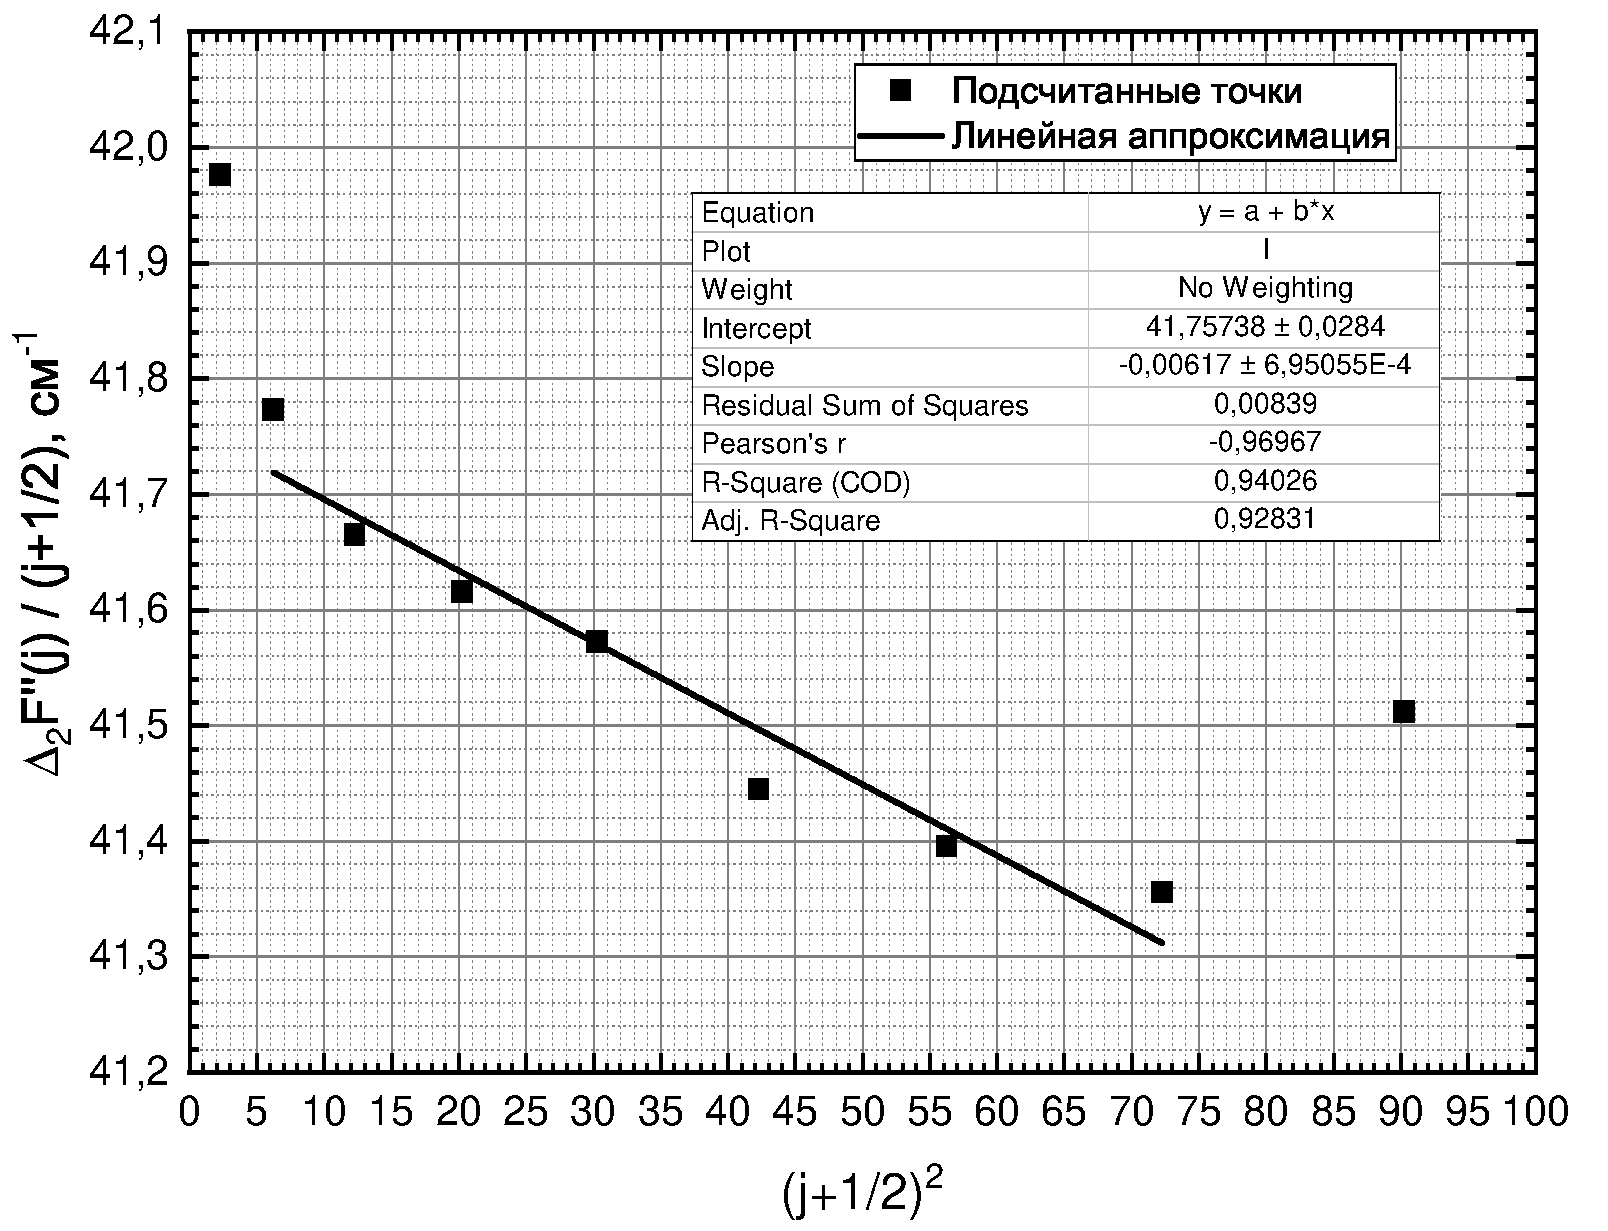
\includegraphics[height=0.49\textheight]{data/delta_F''_j_sq}
	\vspace{-0.2cm}
	\caption{Приведенная комбинационная разность $\Delta_2F''(j)$}
	\label{deltaF''_j}
\end{figure}

Наблюдаемая зависимость сильно отклоняется от линейной. Мы попробуем построить МНК через те точки, которые лучше всего ложатся на прямую. В \textit{первом} случае выкинем первую и две последние точки, во \textit{втором} -- две первых точки и последнюю (см. графики). По построеным зависимостям
% TODO: ДОДЕЛАЙ ЭТО днем. Сейчас 4:32 и я устал
получим молекулярные константы:
\begin{equation}
B_0 = \dfrac{40.571 \pm 0.03}{4} \text{ см}^{-1}
= 10.143 \pm 0.008 \text{ см$^{-1}$}
\end{equation}
% - slope/8
\begin{equation}
D_0 = (0.93 \pm 0.10) \cdot 10^{-3} \text{ см$^{-1}$}
\end{equation}
\begin{equation}
B_1 = \dfrac{41.757 \pm 0.03}{4} \text{ см}^{-1}
= 10.439 \pm 0.008 \text{ см$^{-1}$}
\end{equation}
% -slope/8
\begin{equation}
D_1 = (0.77 \pm 0.09) \cdot 10^{-3} \text{ см$^{-1}$}
\end{equation}
% TODO: уже 4:45. Добей это завтра
% Нет уж, пусть это будет сегодня
\begin{equation}
B_0 = \cfrac{h}{8\pi^2\mu r_0^2c} \Longrightarrow
r_0 = \sqrt{\cfrac{h}{8\pi^2\mu B_0 c}} = 1.25 \text{ \AA}
\end{equation}

\subsection{Воздух}
Изобразим спектр воздуха из легких (рис. \ref{air_co2}). На спектре видны участки, характерные для спектра воды и CO$_2$.
\begin{figure}[H]
	\centering
	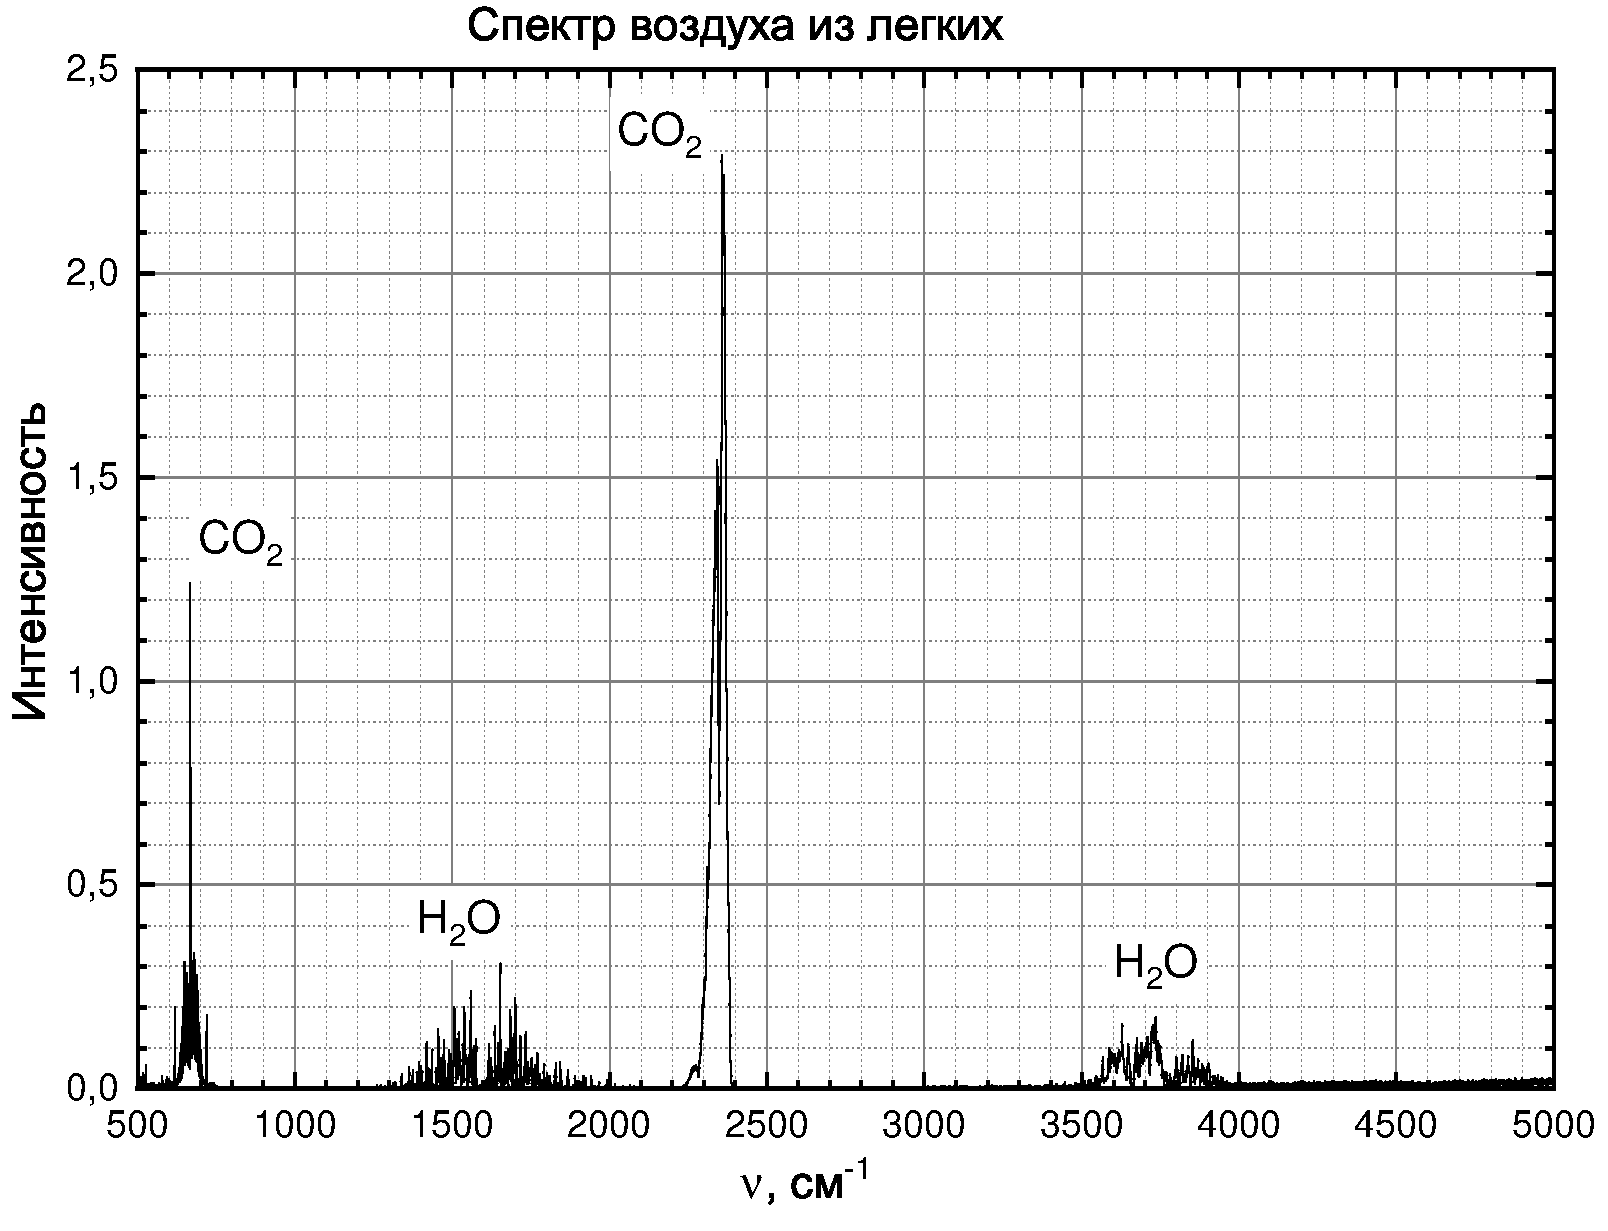
\includegraphics[angle = 90, height=0.95\textheight]{data/dihaniye}
	\caption{ИК-спектр воздуха из легких}
	\label{air_co2}
\end{figure}
\subsection{Неизвестные вещества}
Изобразим спектры, предложенные на анализ. На спектрах отмечены характерные пики, которые позволили определить анализируемое вещество (рис. \ref{ethanol}, \ref{isopropanol}).

Для того, чтобы точно убедиться в справедливости анализа, изобразим спектры этанола и изопропила (рис. \ref{ethanol_real}, \ref{propanol_real}), взятые с электронного ресурса (\href{https://sdbs.db.aist.go.jp/}{https://sdbs.db.aist.go.jp/}).
\begin{figure}[H]
	\centering
	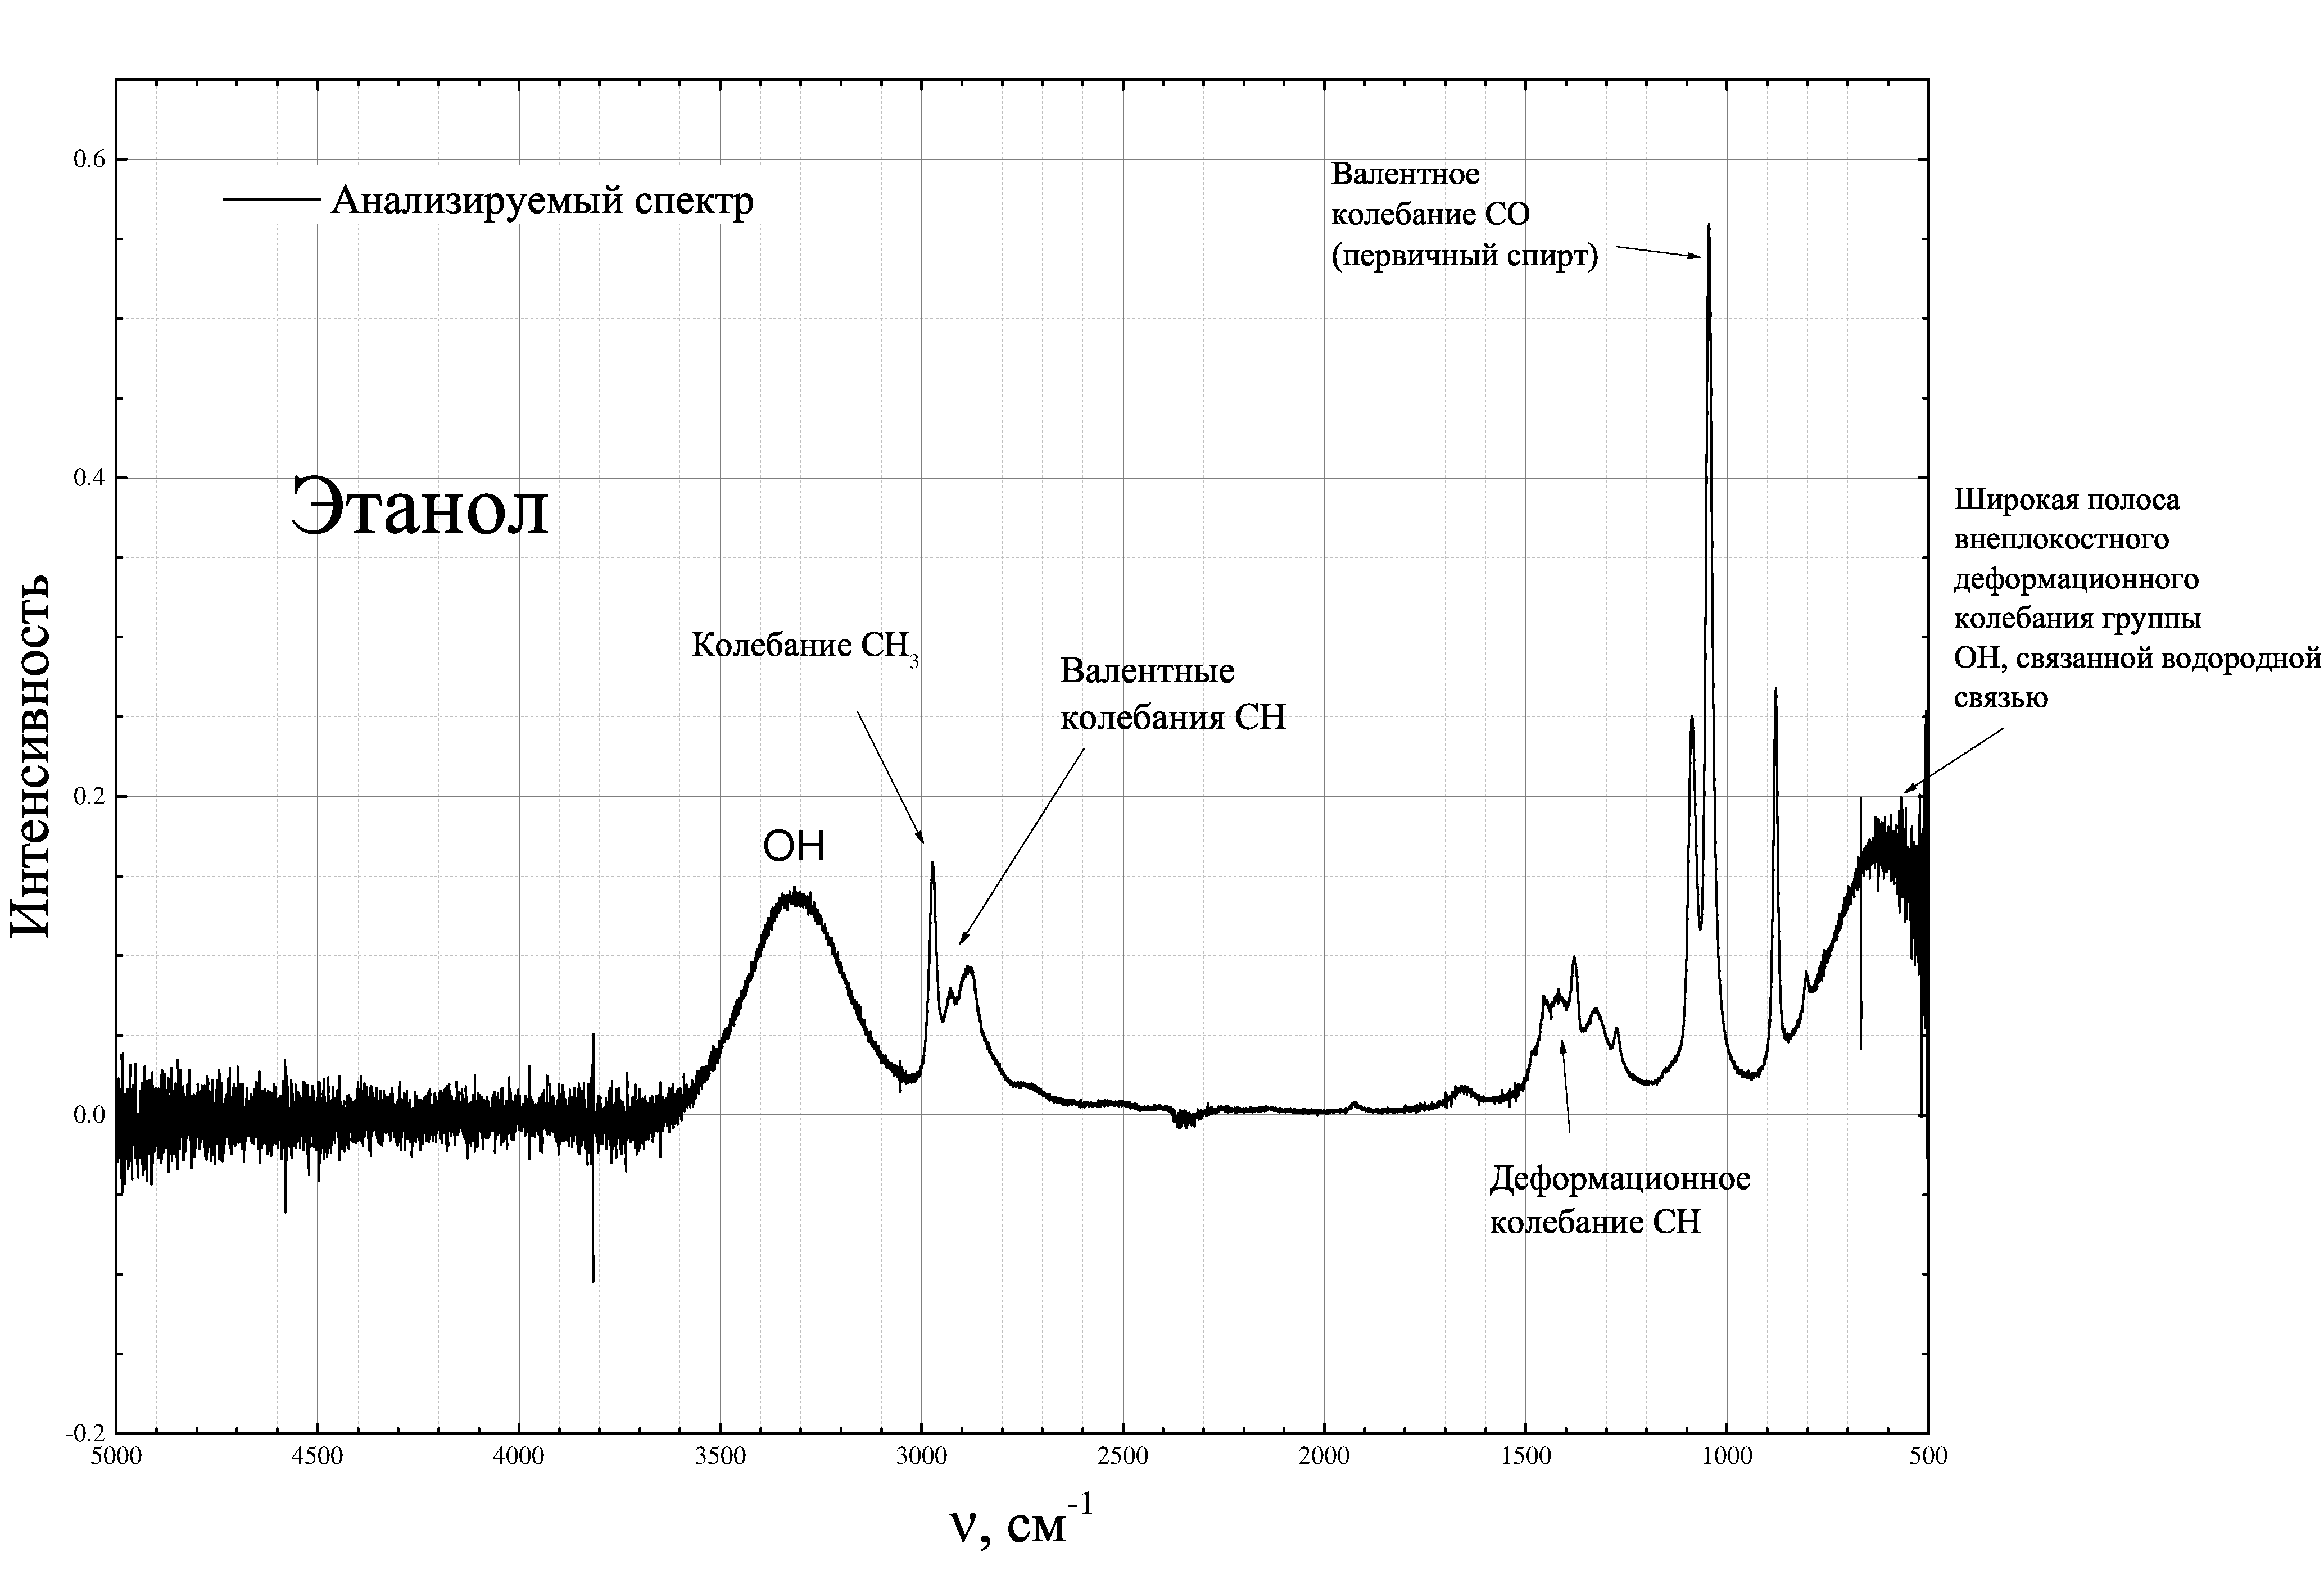
\includegraphics[angle = 90, height=0.83\textheight]{data/ethanol}
	\caption{Неизвестное вещество 1 (этанол)}
	\label{ethanol}
\end{figure}
\begin{figure}[h!]
	\centering
	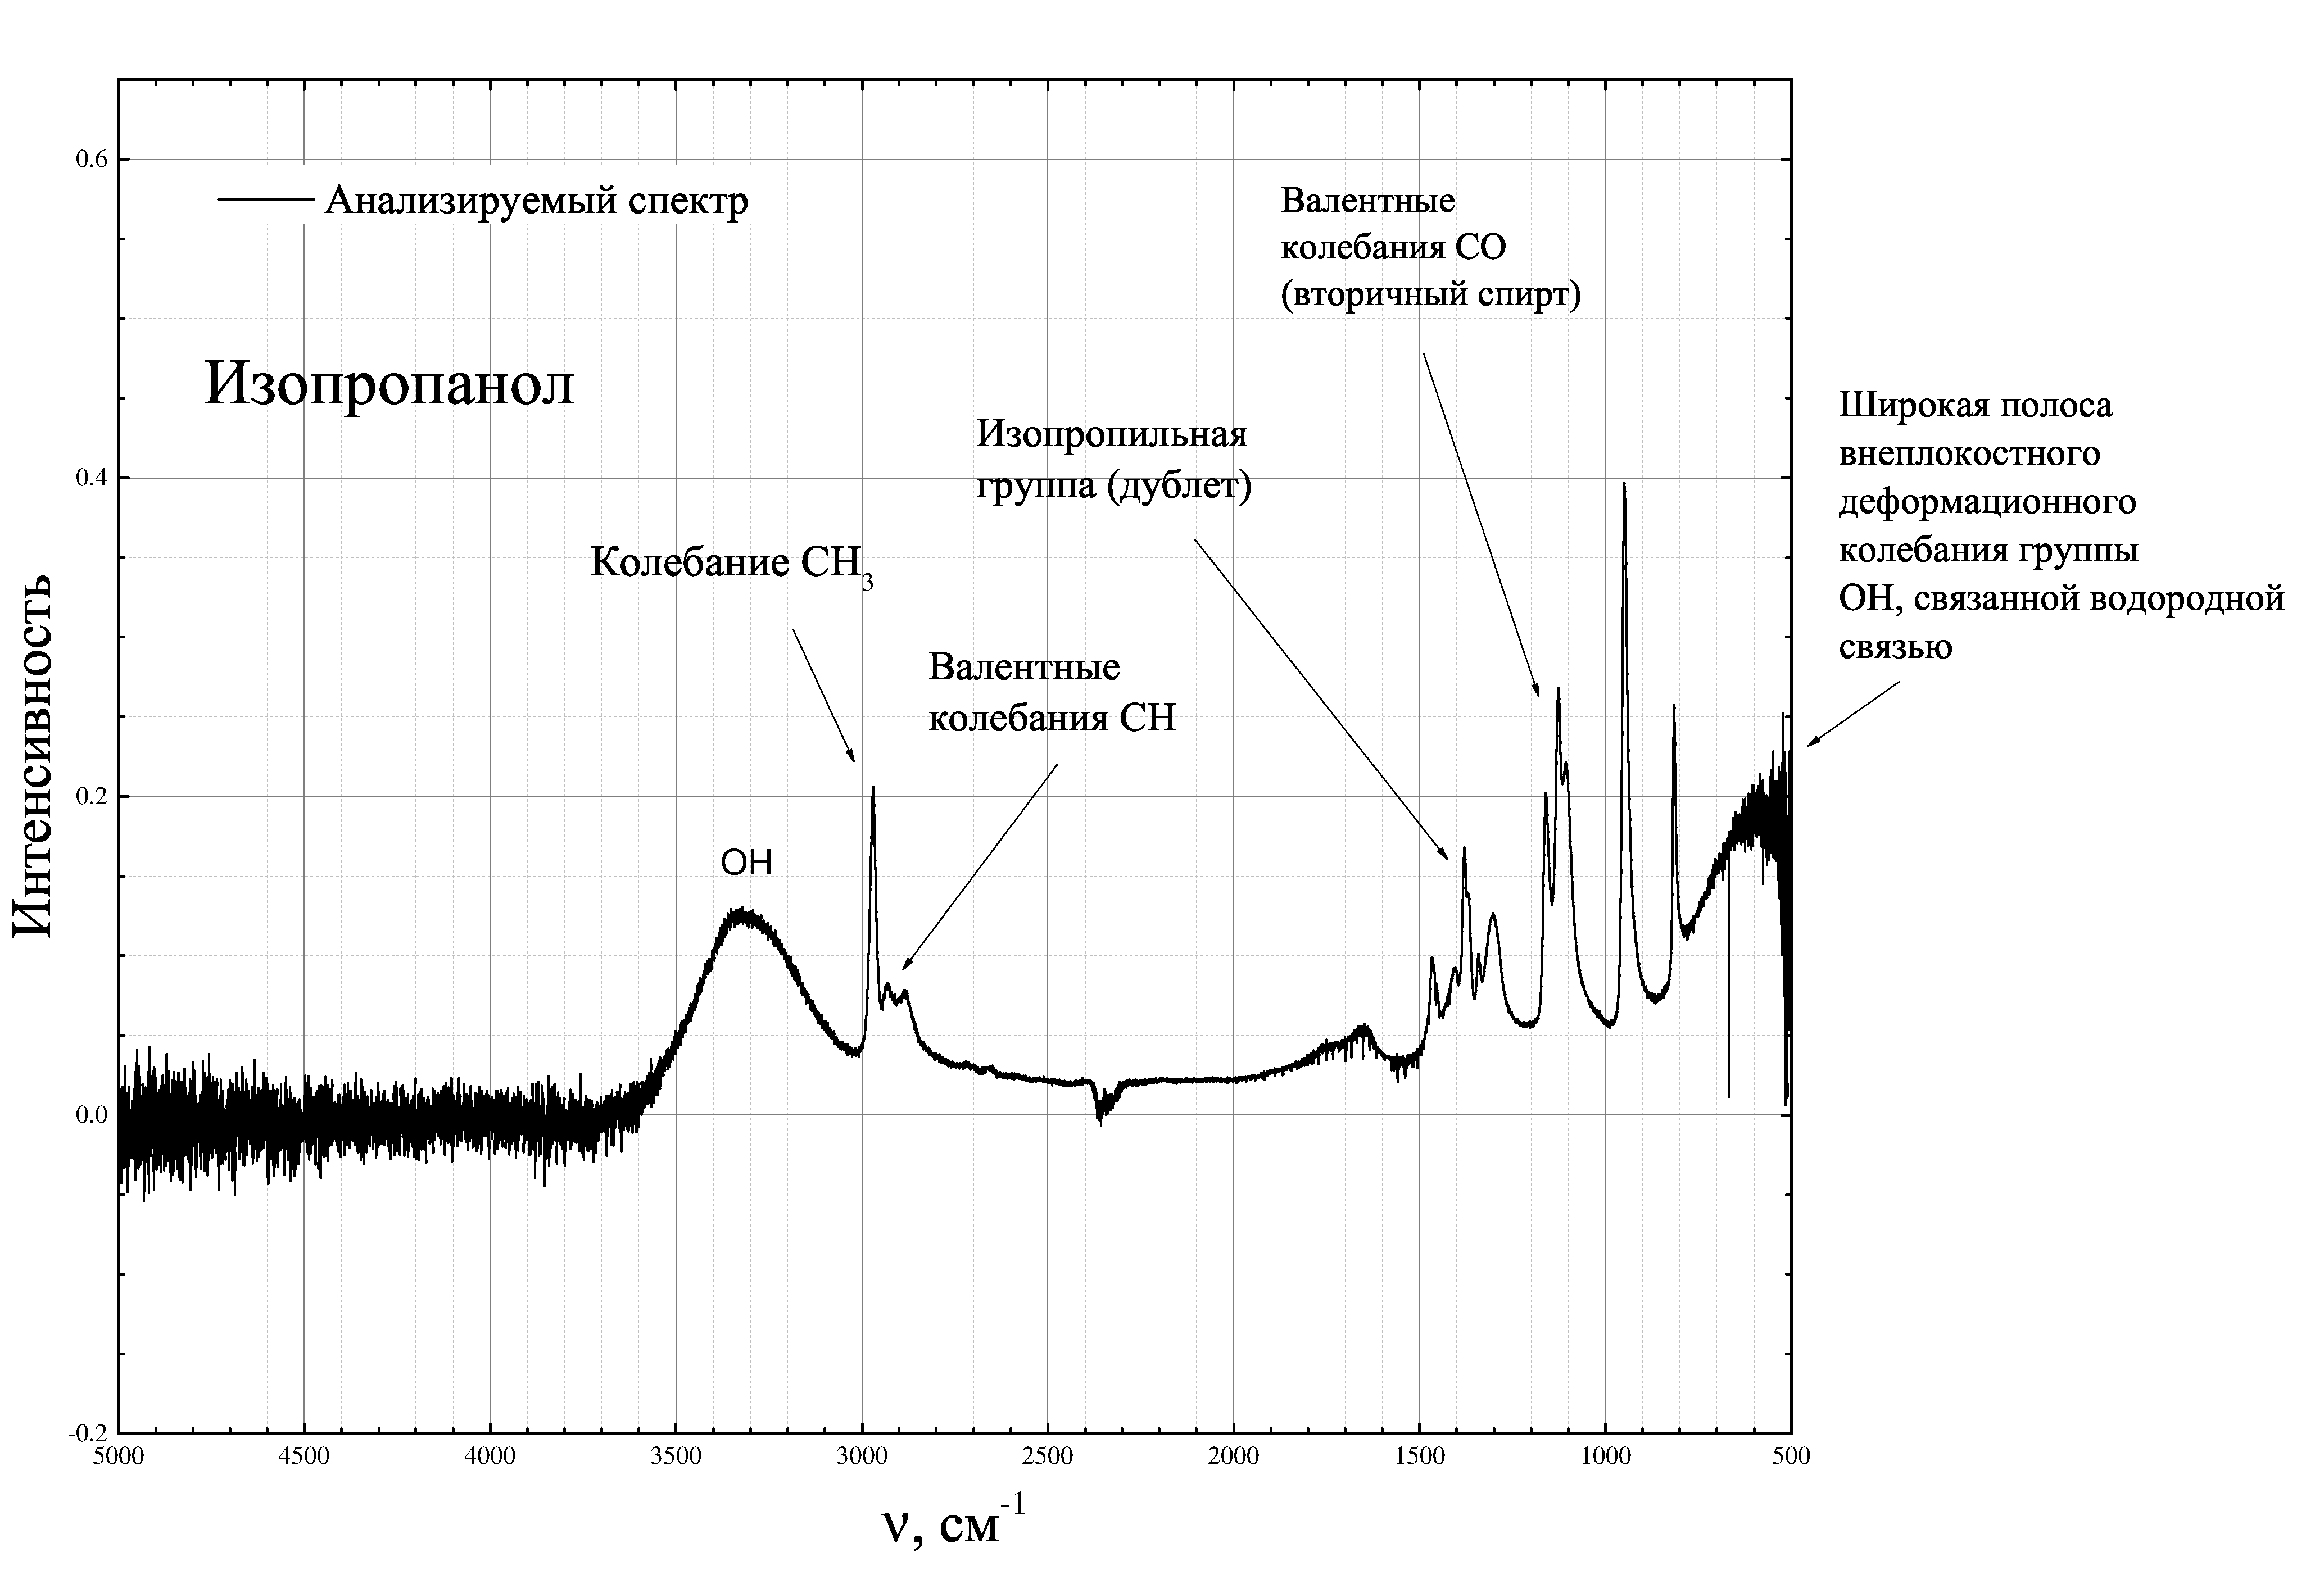
\includegraphics[angle = 90, height=0.95\textheight]{data/isopropanol}
	\caption{Неизвестное вещество 2 (изопропанол)}
	\label{isopropanol}
\end{figure}
\begin{figure}[h!]
	\centering
	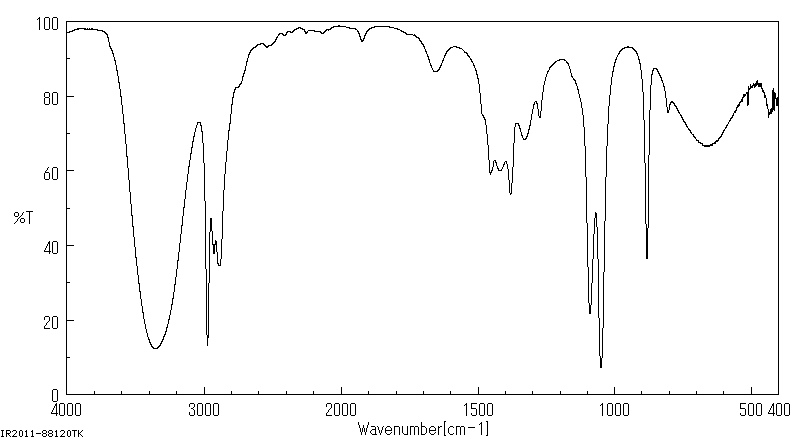
\includegraphics[width=0.9\textwidth]{data/ethanol_real}
	\caption{ИК-спектр поглощения этанола}
	\label{ethanol_real}
\end{figure}
\begin{figure}[h!]
	\centering
	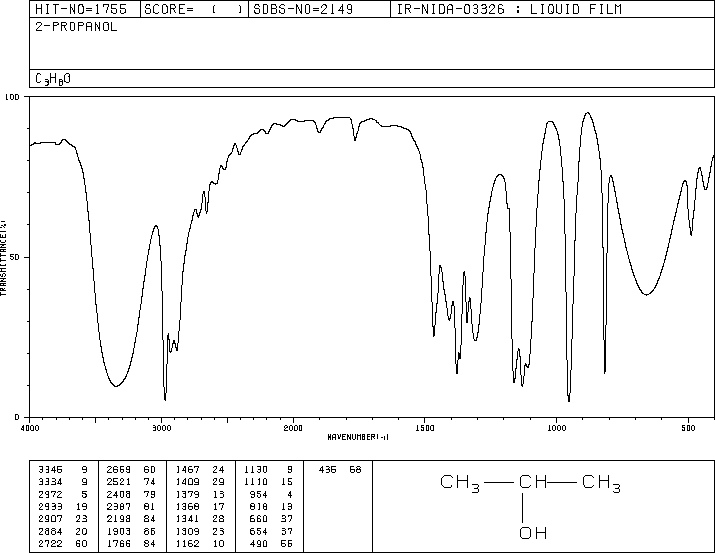
\includegraphics[width=0.9\textwidth]{data/propanol_real}
	\caption{ИК-спектр поглощения изопропанола}
	\label{propanol_real}
\end{figure}
